\documentclass[12pt]{article}
\usepackage[utf8]{inputenc}
\usepackage[T1]{fontenc}
\usepackage{hyperref}
\usepackage{setspace}
\usepackage{mathptmx}
\usepackage{fancyhdr}
\usepackage[english]{babel}
\usepackage[autostyle=true]{csquotes}
\usepackage[letterpaper,margin=1in]{geometry}
\usepackage[style=apa,backend=biber]{biblatex}

\usepackage{siunitx}
\usepackage{graphicx}
\usepackage{titlesec}
\usepackage{multimedia}
\usepackage{indentfirst}

\addbibresource{sources/references.bib}

\doublespacing

\setlength{\parindent}{0.5in}
\begin{document}
  \begin{center}
    \vspace*{\fill}

    \textbf{Investigation into Hemp Hurd-Salt Mixtures for Road De-Icing}
    \vspace{4em}

    Julian Joaquin \\
    Department of Engineering, University of British Columbia \\
    APSC 171: Engineering Drawing and CAD/CAM \\
    Dr. Ray Taheri \\
    December 2nd, 2022

    \vspace*{\fill}
  \end{center}

  \newpage
  \section*{Introduction}
Road salt is commonly used during the winter, preventing both pedestrians and vehicles to safely move over frozen roads.
It is estimated that, of the 54,000,000 metric tons of salt that was consumed in 2021, 42\% of it was used for road deicing \parencite{USG22}.
Such major use of salt has had a significant impact on local ecosystems by increasing the salinity of waterstreams, threatening the state of the surrounding environment \parencite{KGW20}.
Notably, excess salt can enter lakes and rivers, significantly reducing their biodiversity \parencite{HKM22}.
Additionally, salt can also enter fresh drinking water, increasing the salt content such that it meets up to 33\% of an adults recommended daily intake \parencite{CGR22}.
Road salt also leads to damages on infrastructure, costing an estimated \$5 billion in repairs in the U.S. \parencite{EPA20}.

The affects of road deicing have been known for some time now, and many municipalities have investigated reducing the usage of salt.
A common tactic is to pre-wet road salt such that vehicle tires do not throw salt off roads \parencites{ZAS20}{UFK17}.
Other techniques include using a salt-sand mixture to increase road abrasion, creating biodegradable mixtures, and making porous pavement parking lots \parencite{EPA20}.
More recently have biodegradable mixtures been explored as suitable alternatives to salt for road deicing.
One such mixture suggests combining salt with hemp hurd, proposed originally by high school students in Manitoba \parencite{KAV21}.
This mixture is significant compared to other alternatives because it utilizes and promotes the locally growing hemp industry within the province.

Therefore, this study aims to identify the ideal mixture of hemp hurd and salt that works as an affective alternative to traditional road salt.
According to an article written by the CBC, the students found that ``a third of the salt mixed with hemp hurd successfully melted ice nearly as much as salt on its own'' \parencite{KAV21}.
Our investigation will be a repeat of the study done by Bain, Gamayo, and Morant of sorts, where we will focus on testing for the ideal ratio of salt-hemp based on its effectiveness in de-icing.

  \section*{Background}

Deicers are predominantly composed of sodium chloride, or salt.
A sodium chloride solution with water has a higher freezing point than a pure water liquid.
Hence, when it is dissolved into the ice on roads, the ice melts into water.
Some consumer-grade deicers also contain calcium chloride, which creates an exothermic reaction upon contact with water.
This makes it quicker at deicing than sodium chloride, and an appropriately balanced mixture of both compounds can result in an effective and environmentally safer mixture since less overall substance is used.
However, on larger scales, using a calcium chloride--sodium chloride mix is uneconomical so calcium chloride is not used for city-wide deicing.
The same can be said for other deicing compounds, either due to difficult sourcing or extraction \parencite{ARF15}.

Alternatively, some cities will try to increase the traction on roads using sand.
It is easy to source in most places while being cheap and abundant.
However, the sand is often pushed off the roads in the spring, creating lasting sediment that can clog in waterways and basins, requiring huge investment to clean up and maintain \parencite{EPA20}.
The use of biodegradable deicing mixtures is therefore appealing, since they should have a lower environmental impact and could potentially utilize agricultural byproducts.
Bain, Gamayo, and Morant explored this idea by testing several agricultural byproducts that were local to Manitoba, and found that hemp hurd was particularly effective in supplementing sodium chloride for deicing \parencite{KAV21}.
Specifically, the hemp hurd was effective in absorbing the escaping moisture while also providing a degree of traction.
Additionally, considering the growing hemp industry in Canada, the use of hemp hurd can be seen as an effort to increase the utility output of hemp plants and reduce waste in production.
As such, the mixture was presented to Winnipeg's city council as a solution to reducing the amount of salt used on roads every winter.


  \section*{Method}

Our experiment for determining the ideal mixture involves 5 sample mixtures and one control mixture (which will just be salt).
The sample mixtures will have the following volumetric ratio of hemp to salt: 1:1, 2:1, 3:1, 4:1, and 5:1, and will contain a third of the salt of the control mixture. 
The samples of each mixtures will be called sample 1 through 5, respectively.
With consideration for the size of the containers, control sample will have \SI{15}{\ml} of salt.
Thus, each experimental sample will have \SI{5}{\ml} of salt and their respective amount of hemp hurd.
The ice will be grown in small food storage containers in overnight winter conditions.
Once the water inside the containers is fully frozen, each mixture will be applied to the exposed ice surface.
Observations on the performance of the mixtures will be taken for 90 minutes after its application.

There will be 2 different trials for testing each mixture.
Due to constraints in equipment, the deicing effectiveness of each mixture will be measured by visual observation.
The visual observations will be recorded through filming by a camera.
The first trial will look at the performance of each mixture by visually observing their effectiveness with \SI{2}{\mm} thick ice you could expect after a light snowfall.
This includes observing how much ice is melted, the amount of water present after a certain amount of time, and other characteristics that aid in the removal of ice.
The second experiment looks at a worse case scenario where the ice is unquantifiably and unrealisticly thick.
It is expected that no mixture will work effectively with this test, the approximate amount of ice that is melted will be the primary characteristic to observe.

  \section*{Results}

\begin{figure}[t]
  \centering
  \label{mov:trial1}
  \movie[externalviewer]{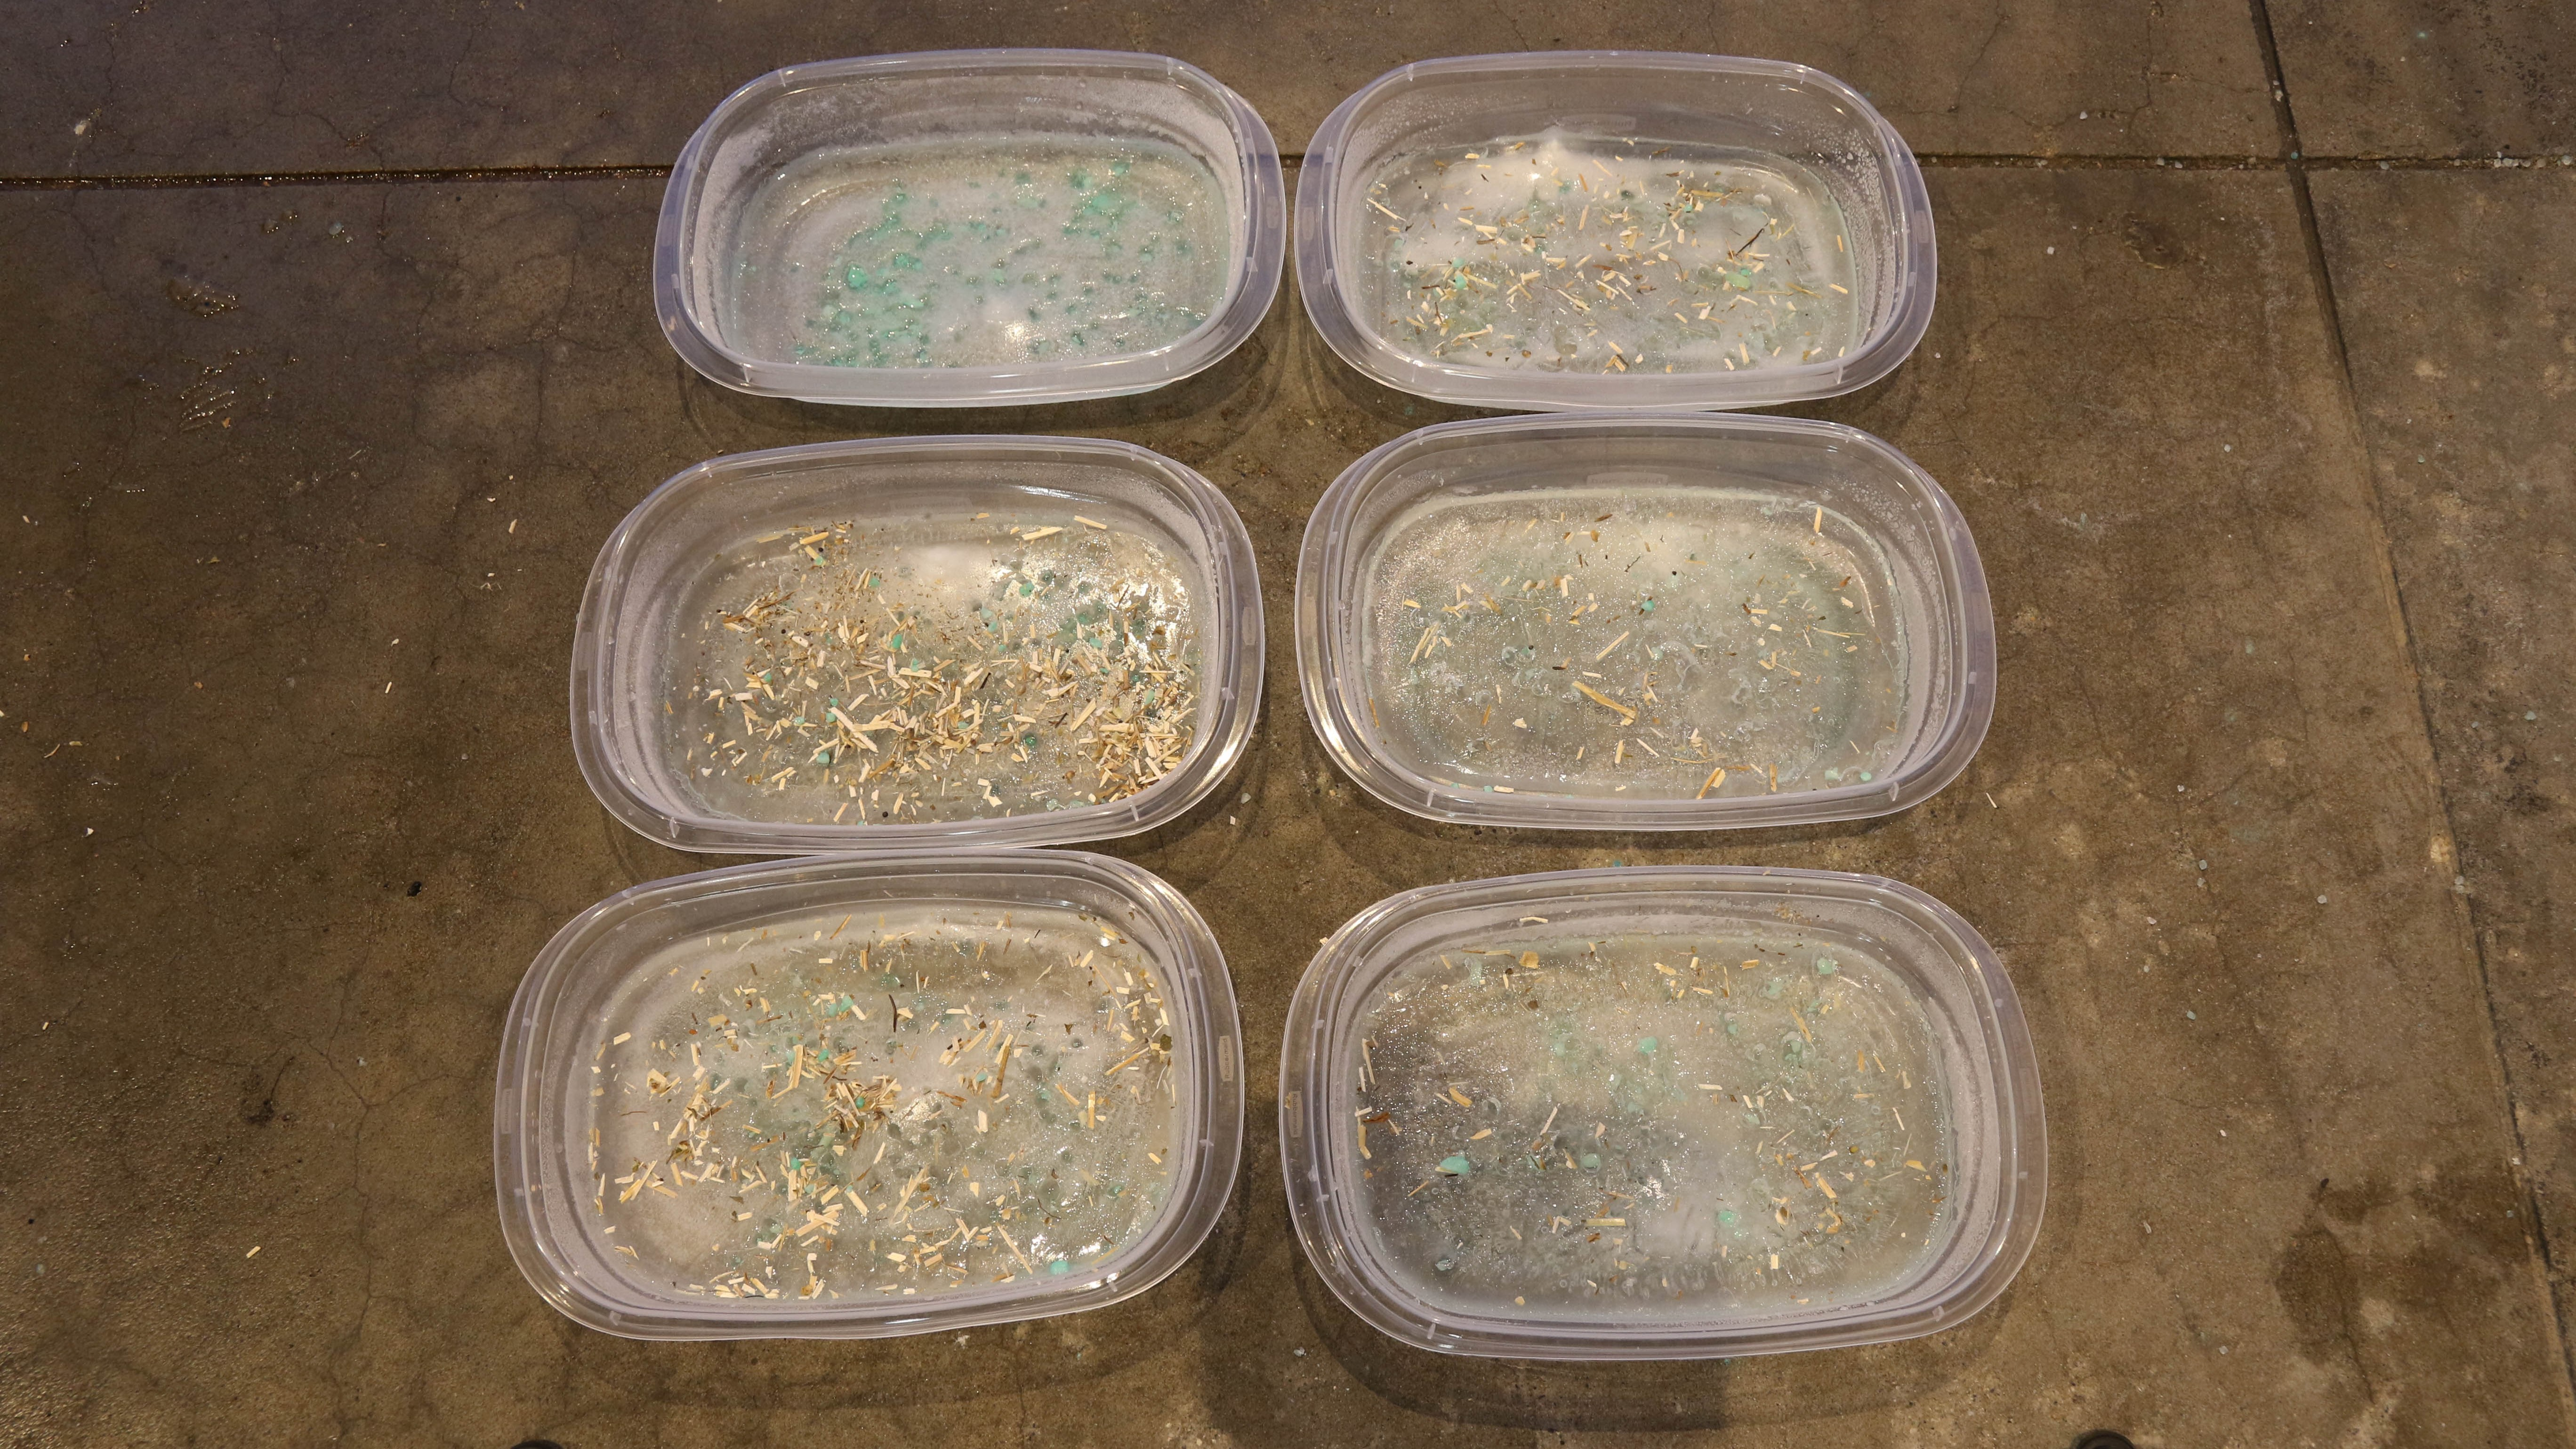
\includegraphics[width=\textwidth]{assets/icetest2-505.jpg}}{ice-timelapse1-compressed.mp4}
  \caption{\small Timelapse of trial 1. Samples are ordered 1--5 plus the control sample, from bottom to top on both columns, starting with the lowest rightmost column of containers. This video corresponds with the \texttt{ice-timelapse1-compressed.mp4} file provided with this report.}
\end{figure}
The first trial was performed in \SI{-8}{\degreeCelsius} weather.
Due to external circumstances, the trial could only be conducted for 60 minutes.
The timelapse can be viewed through \hyperref[mov:trial1]{Figure 1} as embedded multimedia.\footnote[1]{Adobe Acrobat Reader version 6 or later is \textbf{required} in order to play the timelapse through the PDF. By clicking the figure, Acrobat Reader will prompt to open the respective video file, to which the timelapse will play through the default video player on your system. Alternatively, you can view the video through the provided \texttt{.mp4} files.}
An additional small quantity of salt is added to each sample after 30 minutes because of lower effectiveness than expected.
The mixtures performed as expected of a deicing salt agent; all, to some degree, melted some of the ice and water could be seen accumulating at the bottom of the containers.
The control sample became notably porous within 15 minutes after applying the salt.
Once reaching the bottom of the container, the salt began to dissolve into the aforementioned water.
This resulted in the ice partially dislodging from the bottom of the container and was observed with the other samples in the trial.
All samples showed the same degree of increasing ice asperity in the duration of the experiment and demonstrated a degree of perforation from the salt.
Samples 1 and 2 were mildly perforated by the salt, undermined by latent refreezing after some time.
By contrast, sample 3--5 were moderately perforated and did not see any latent refreezing.
This is attributed to the absorption of the volume of hemp hurd, as it prevents the resulting water to refreeze.
While the control sample undoubtedly melted a greater volume of ice, the experimental samples showed a comparable amount of melting to a degree that is not insignificant.

\begin{figure}[t]
  \centering
  \label{mov:trial2}
  \movie[externalviewer]{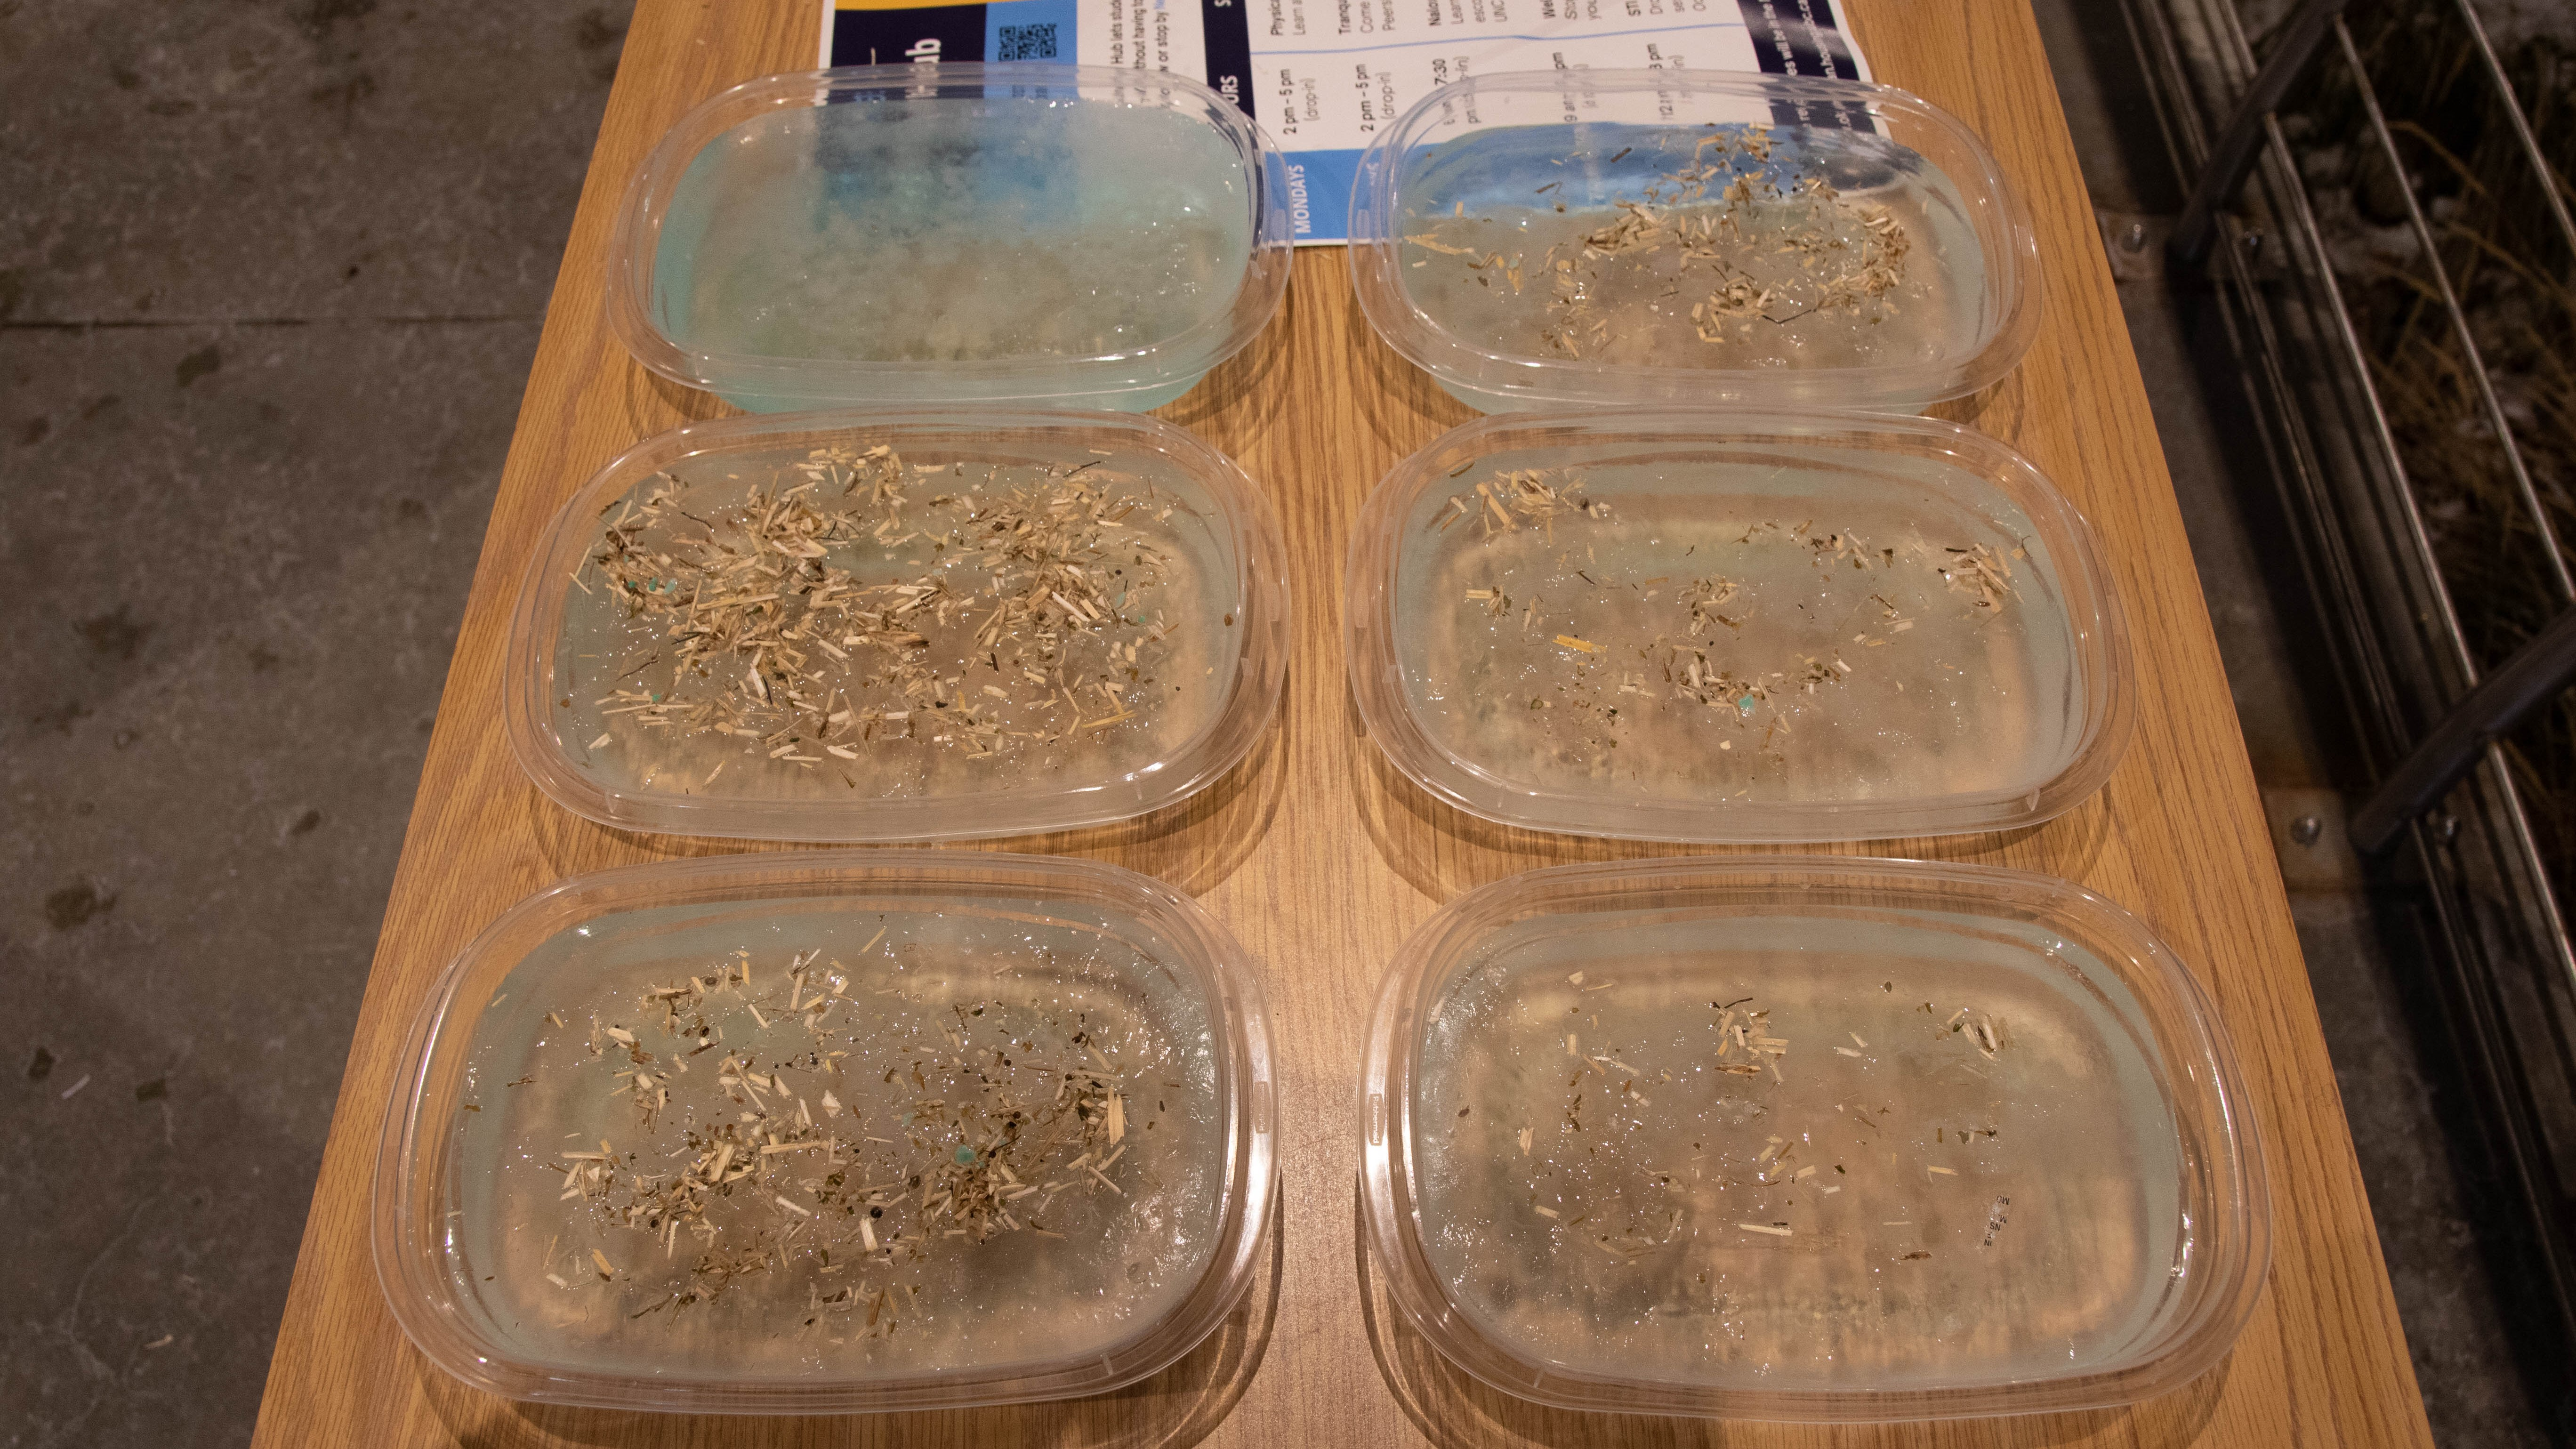
\includegraphics[width=\textwidth]{assets/icetest-800.jpg}}{ice-timelapse2-compressed.mp4}
  \caption{\small Timelapse of trial 2. Samples are ordered 1--5 plus the control sample, from bottom to top on both columns, starting with the lowest rightmost column of containers. This video corresponds with the \texttt{ice-timelapse2-compressed.mp4} file provided with this report.}
\end{figure}

The second trial was performed in \SI{-2}{\degreeCelsius} weather and conducted for 90 minutes.
Due to challenges in producing the ice for this trial, there was a significant amount of water \SI{5}{\mm} below the ice surface, a lesser thickness than what was originally intended for this trial.
The consequence resulted in the salt crystals completely dissolving after going through the \SI{5}{\mm} of ice.
The ice melted quicker than expected after application, likely due to the relatively warmer ambient temperature.
An additional small quantity of salt is added to each sample after 30 minutes because less ice was melted than expected.
Differences outstanding, the results were similar to the first trial.
Samples 1 and 2 showed some amounts of perforation and asperity, while 3--5 showed moderate amounts.
The control sample was heavily perforated and appeared likely to shatter with some pressure after 90 minutes had elapsed.
The perforation of the samples reduced the integrity of the ice, as found during the disposal of the samples.
Lastly, the hemp in all experimental samples seemed to infuse with the ice, becoming embedded in the surface.


  \input{sections/4-discussion.tex}

  \input{sections/5-conclusion.tex}

  \newpage

  \printbibliography
\end{document}